% ----------------------------------------------------------
% PARTE
% ----------------------------------------------------------
\part{Resultados}
% ----------------------------------------------------------

\section{Kaggle}

Kaggle é uma plataforma criada em 2010 que reune ferramentas e estudos sobre modelagem preditiva. Também viabiliza competições de temas relacionados a análise preditiva. Com o intuito de compartilhar conhecimento, qualquer interessado pode acessar dados de empresas para aplicar estudos ou gerar novos modelos. Além disso, o Kaggle também tem sido usado como uma forma de recrutar cientistas de dados. 


\subsection{Loan Club}

A Loan Club é um marketplace de créditos online. Trata-se de uma plataforma que reune pessoas que gostaria de realizar um empréstimo e outras que possuem um capital a investir. Em geral, são empréstimos pessoas, de negócios ou para procedimentos médicos. A proposta é oferecer um serviço de fácil acesso via dispositivos mobiles a taxa baixas, além de garantir um retorno que se ajuste a expectativa do investidor. Dessa forma, operam de forma menos burocrática do que um banco, mas assumindo os riscos de uma instituição financeira.


\section{Tecnologias}

\subsection{Scikit Learn}

O scikit é um framework desenvolvido em Python voltado para data science. Possui implementação de diversos algoritmos e de ferramentas que auxiliam desde a análise dos dados até na execução de tarefas como clusterização e classificação até a execução dos algoritmos de machine learning. Possui integrações com programas visuais (como será mostrado a seguir). Já são mais de 30 contribuidores ativos.


\subsection{Apache Spark}

O Apache Spark é uma ferramenta que resolve um problema relacionado a escalabilidade da execução de algoritmos de machine learning. Os 3 algoritmos estudos (em especial o Kmédias) possui uma carga de contas alto. Para bases grandes, aspecto relevante quando se trata de Big Data, o scikit não é capaz de executar em tempo hábil. O Apache Spark, por outro lado, oferece uma solução robusta para a execução dos algoritmos de machine learning. Embora seja possível configurá-lo para que os algortimos sejam executados em tempo real com alimentação contínua de dados, tal abordagem não será contemplada por não se tratar do foco do estudo.

\section{Algoritmos}

\subsection{Preparação da base}

Como uma base de uma empresa, o Loan Club apresenta diversos problemas como:

\subsection{Missing values}
Inerente a uma base comum de qualquer empresa, missing values ocorre quando uma informação não consta na base. Esse fato pode influenciar a conclusão de uma análise porque a ausência de dados pode distorcer qualquer análise. Para diminuir o impacto desse tipo de problema, é necessário verificar a natureza da informação. Elas são oriundas desde problemas do armazenamento da informação, provenientes desde erros humanos, falta de informação ou em decorrência de algum problema ou inconsistência no sistema de informação.

Para os algortimos, é necessário que algum valor seja colocado para a realização das cálculos dos algoritmos. Há diversas abordagens, como subustituição por um valor padrão que faça sentido para cada informação. Em alguns casos, são usados valores como 0, média ou moda das observações. Contudo, é evidente que cada uma dessas técnicas enviesa e modifica o resultado. Neste estudo, desprezamos as informações que possuiam altas ocorrências de missing values e para as que possuiam menos de 1\% de missing values, foi preenchido com 0.

\subsubsection{Necessidade de tratamentos de dados}
Alguns dados como intrate ou o term estavam armazenados como tipo texto, sendo inviável a execução do algoritmo do k médias.

\subsubsection{Normalização de dados}



\subsubsection{Remoção das variáveis categóricas}

\subsection{K Médias}

O objetivo de uma clusterização é para dado um conjunto de objetos, colocar os elementos em grupos baseados na similaridade entre eles. Neste trabalho, a idéia é encontrar padrões inesperados nos
dados, por se tratar de um problema que não está totalmente claro.

O diagrama de Voronoi é uma ferramenta utilizada para visualizar problemas que envolvem conceito de proximidade em um plano. Baseia-se no fato de que em um plano, existem pontos que estão mais próximos de uma fonte geradora do que de outra fonte, o resultado é um polígono de cujas distâncias entre a fonte e ponto são as menores possíveis (MOURA, 2003). Portanto, é possível ter uma visualização espacial da distribuição dos registros, bem como os centróides.

\begin{figure}[!ht]
\caption{Visualização dos pontos no diagrama de Voronoi com os dados sem normalizacao}
\centerline{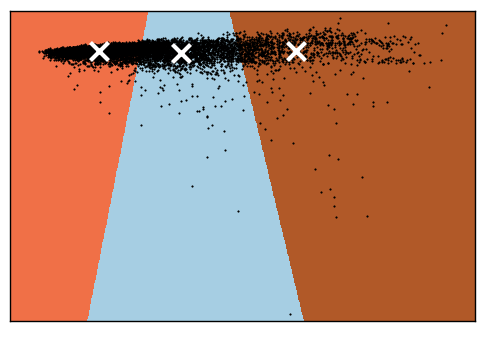
\includegraphics[width=0.5\textwidth]{img/voronoi}}
\fonte{Gerado a partir do script}
\end{figure}

A imagem mostra um diagrama de Voronoi. Os polígonos externos se estendem infinitamente no plano, logo são desenhados como figuras abertas. Cada aresta do diagrama constitui um lugar onde os pontos são equidistantes em relação à dois locais. Os vértices dos polígonos estão ligados outras arestas sendo pontos de equidistânciacada região definidas.

Para a visualização desse diagrama, foi necessário realizar uma operação de redução de dimensionalidade de variáveis para 2 features. Neste estudo, aplicamos a construção do diagrama para 8000 registros.

Também é possível fazer uma análise para verificar a quantidade de clusters ideal para a amostragem. A cada execução do algoritmo também foi calculado um score chamado sillhouette, que é uma forma de interpretar e mensurar a validação da consistência dos clusters, além de fornecer uma representação gráfica de quão bem os dados estão inseridos nos clusters (coesão) em comparação a outros (separação). Esse score varia de -1 a 1, na qual quanto mais próximo de 1, mais bem encaixado encontra-se o elemento com seu respectivo cluster.

\begin{figure}[!ht]
\caption{Analise para 2 clusters }
\centerline{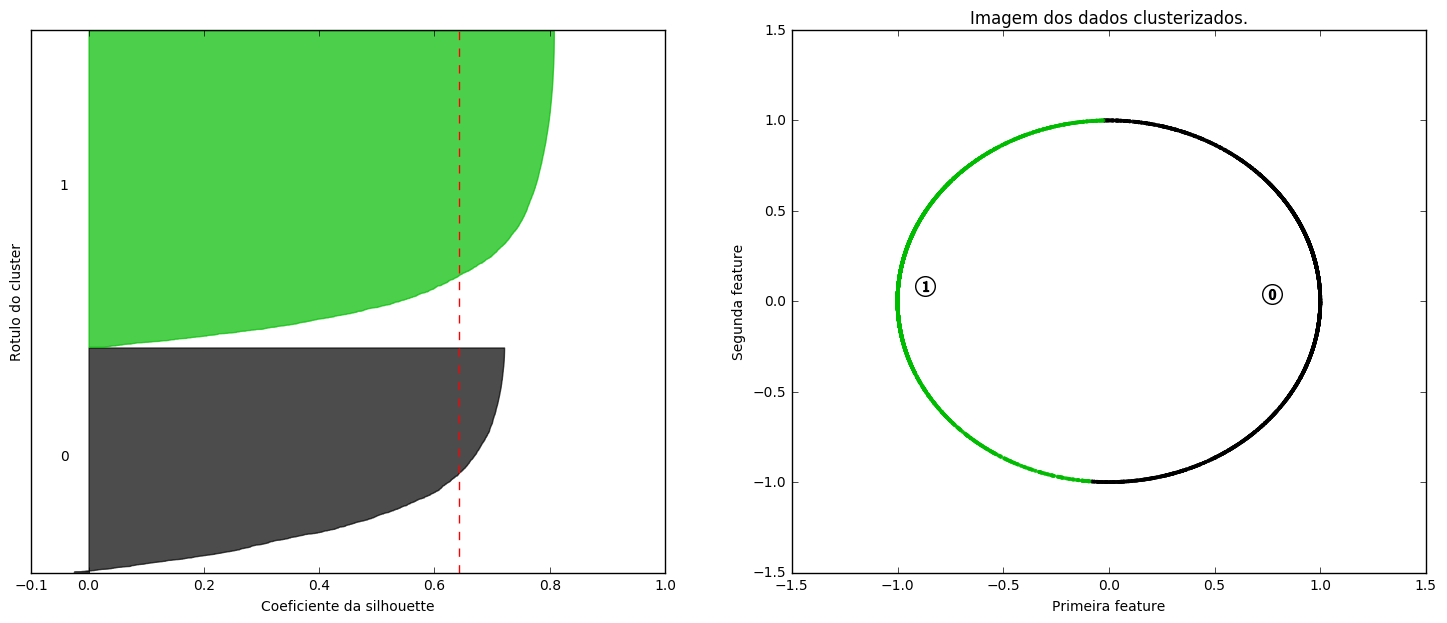
\includegraphics[width=.85\textwidth]{img/silhoute2}}
\fonte{Gerado a partir do script}
\end{figure}

A primeira tentativa foi de separar a amostra em 2 clusters. Para essa divisão, foi obtida um score de 0,6428.


\begin{figure}[!ht]
\caption{Analise dos 3 clusters }
\centerline{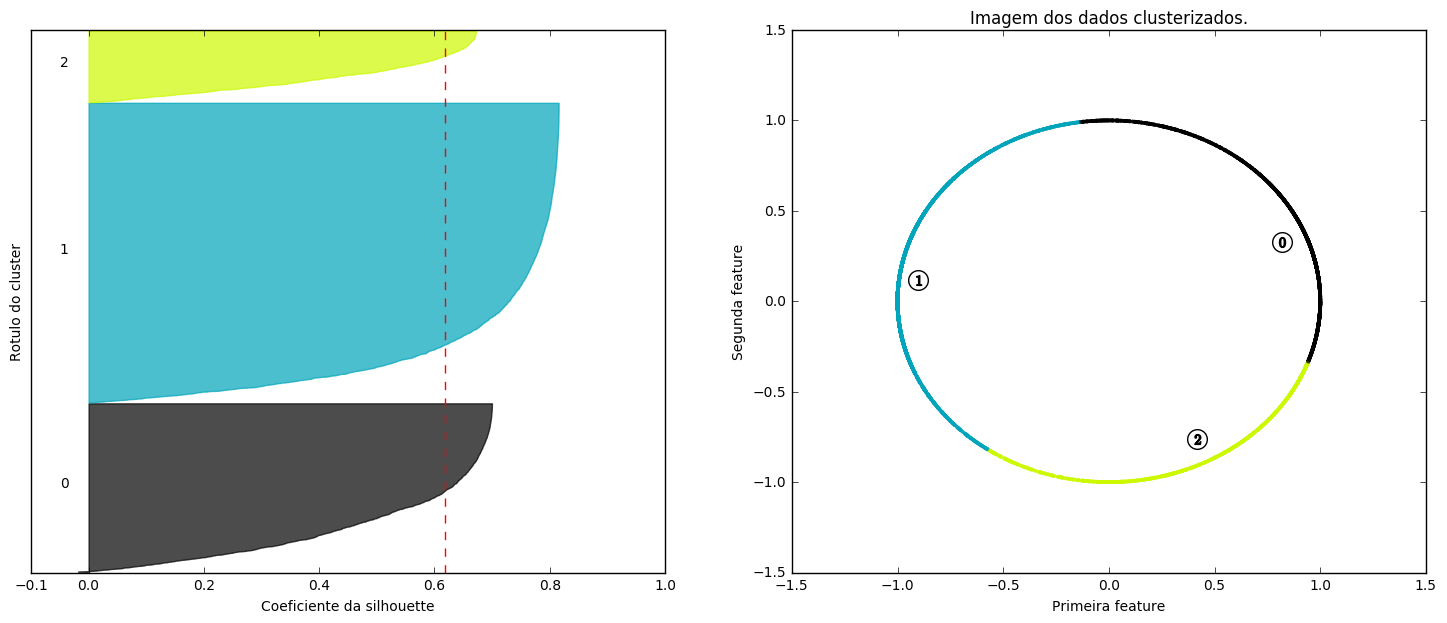
\includegraphics[width=.85\textwidth]{img/silhoute3}}
\fonte{Gerado a partir do script}
\end{figure}

Para a divisão em 3 clusters, foi obtida a nota 0,6188.


\begin{figure}[!ht]
\caption{Analise dos 4 clusters }
\centerline{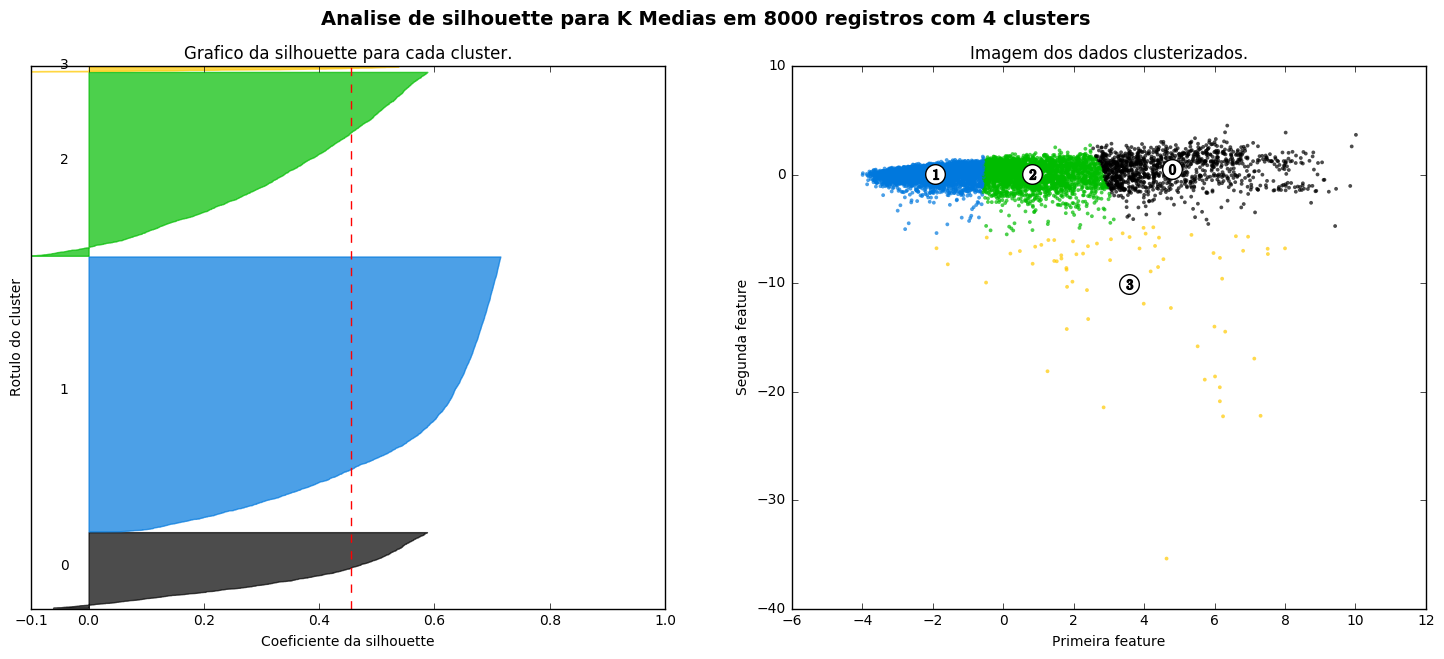
\includegraphics[width=.85\textwidth]{img/silhoute4}}
\fonte{Gerado a partir do script}
\end{figure}

Para a divisão em 4 clusters, foi obtida a nota 0,6099.


A clusterização gerada a partir do K médias servirá de parâmetro para os algoritmos de regressão logística e random forest.


\subsection{Regressão Logística}

A função logistic

\begin{figure}[!ht]
\caption{Funcao logistic para a feature fundedamnt}
\centerline{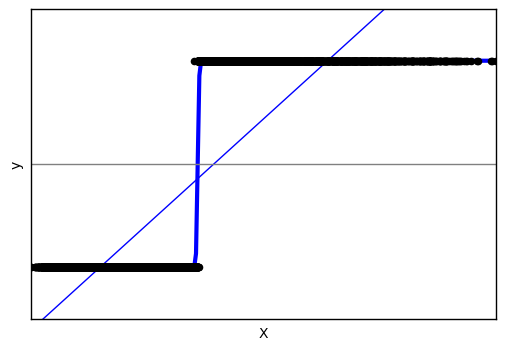
\includegraphics[width=.6\textwidth]{img/logit}}
\fonte{Gerado a partir do script}
\end{figure}

Também conhecida como matriz de erros, a confusion matrix é uma representação visual dos erros ocorridos durante o processamento do algoritmo. As linhas representam a classe que o dado pertence e a coluna representa a classificação gerada durante o processo. Quando um registro não está dentro da diagonal principal, significa que o algoritmo fez uma classificação diferente do que foi esperado.

\begin{figure}[!ht]
\caption{Confusion Matrix}
\centerline{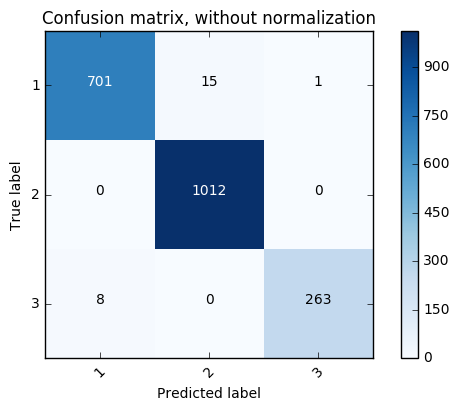
\includegraphics[width=.6\textwidth]{img/confusionMatrix}}
\fonte{Gerado a partir do script}
\end{figure}


Para o caso do Loan Club, podemos notar que a função gerada pela regressão logística possui um indíce de acurácia alto.

\subsection{Random Forest}


Com uma árvore de decisão tem-se uma representação visual, de fácil interpretação de como é feito a classificação. Foi possível construir uma árvore para ilustrar a árvore do Loan Club. Neste caso, foi feito uma redução de dimensionalidade para 2 features, considerando-se 3 clusters.

\begin{figure}[!ht]
\caption{Estrutura da arvore de decisao com dimensionalidade reduzida para 2 features}
\centerline{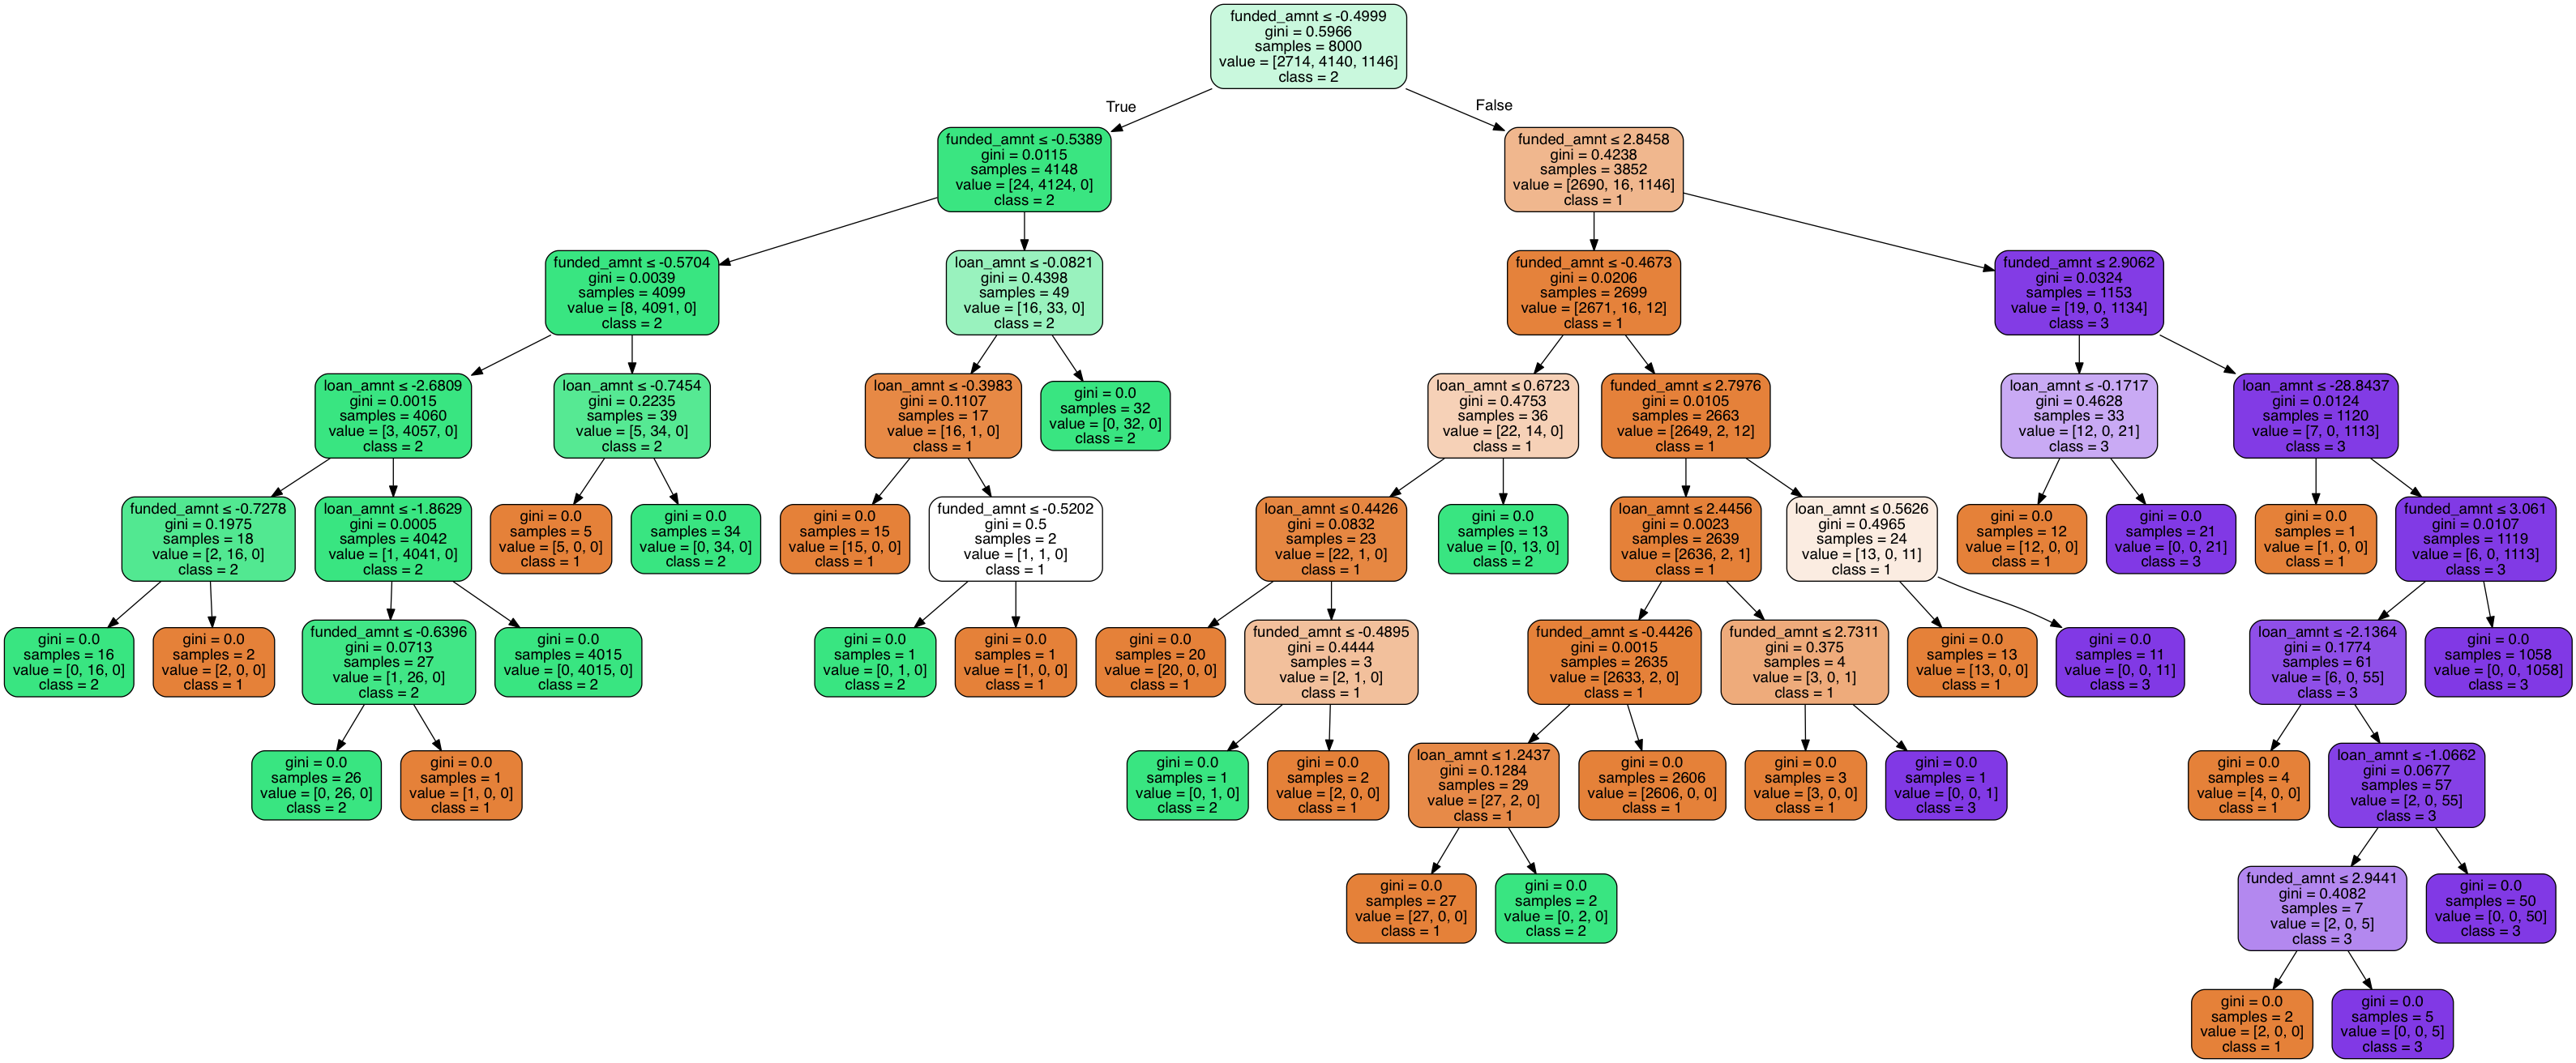
\includegraphics[width=1.05\textwidth]{img/loan}}
\fonte{Gerado a partir do script}
\end{figure}

A árvore para mais de 20 features fica muito maior por conta da quantidade de informações.


Ao gerar uma árvore de classificação, o algoritmo também disponibiliza a relevância das features.

\begin{figure}[!ht]
\caption{Features mais relevantes}
\centerline{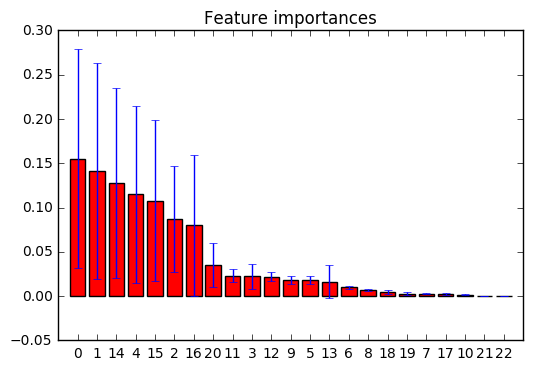
\includegraphics[width=.7\textwidth]{img/tree-most-important-features}}
\fonte{Gerado a partir do script}
\end{figure}

Desta base, é possível notar que 8 destas features possuem maior relevância frente as demais. Isso pode implicar numa redução de dimensionalidade, ocasionando economia de processamento de dados. Por outro lado, isso é válido partindo-se do pressuposto de que a natureza das informações se manterão, o que pode não ser verdade.

%
%\lstinputlisting[language=Python, firstline=37, lastline=45]{
%load_data.py
%}

Assim como foi feito na regressão logística, pode-se calcular a confusion matrix para visualizar a acurácia.

\begin{figure}[!ht]
\caption{Confusion Matrix}
\centerline{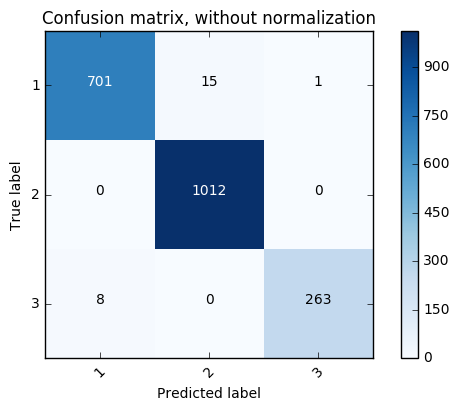
\includegraphics[width=.6\textwidth]{img/confusionMatrix}}
\fonte{Gerado a partir do script}
\end{figure}



% ---
% primeiro capitulo de Resultados
% ---
%\chapter{Lectus lobortis condimentum}
% ---

% ---
%\section{Vestibulum ante ipsum primis in faucibus orci luctus et ultrices
%posuere cubilia Curae}
% ---

%\lipsum[21-22]

% ---
% segundo capitulo de Resultados
% ---
%\chapter{Nam sed tellus sit amet lectus urna ullamcorper tristique interdum
%elementum}
% ---

% ---
%\section{Pellentesque sit amet pede ac sem eleifend consectetuer}
% ---

%\lipsum[24]

% ----------------------------------------------------------
% Finaliza a parte no bookmark do PDF
% para que se inicie o bookmark na raiz
% e adiciona espaço de parte no Sumário
% ----------------------------------------------------------
%\phantompart